\chapter{Обзор теоретической литературы по~криптографии и интернету вещей} \label{ch1}

% не рекомендуется использовать отдельную section <<введение>> после лета 2020 года
%\section{Введение. Сложносоставное название первого параграфа первой главы для~демонстрации переноса слов в содержании} \label{ch1:intro}


\section{Криптографические алгоритмы: основные понятия} \label{ch1:sec1}


\subsection{Информация и криптография} % ~ нужен, чтобы избавиться от висячего предлога (союза) в конце строки

Человеческая цивилизация в течение всего времени существования работает с различной информацией. Информация может представлять собой как исторические сведения или описания технологических процессов, так и частные данные человека или группы лиц. Сведения, составляющие информацию и представляющие определенную ценность, должны быть защищены от лиц, не имеющих соответствующих прав доступа. Поэтому задача защиты информации всегда была актуальной. 

Защитить информацию можно тремя способами \cite{src8}.
\begin{enumerate}
	\item Создание абсолютно надежного и изолированного от доступа извне хранилища информации и инфраструктуры для него. Это является крайне трудоемкой и дорогостоящей задачей.
	\item Скрытие факта существования или передачи информации. Средства и методы такого скрытия изучает стеганография.
	\item Хранение и передача информации, преобразованной таким образом, чтобы обратное преобразование могли совершить только определенные лица. Средства и методы такого преобразования информации изучает криптография.
\end{enumerate} 

Формализуем вышесказанное.

Информация – сведения, передаваемые одними людьми другим людям устным, письменным или каким-либо другим способом, а также сам процесс передачи или получения этих сведений \cite{src9}.

Защита информации – деятельность, направленная на предотвращение утечки защищаемой информации, несанкционированных и непреднамеренных воздействий на защищаемую информацию \cite{src10}. Утечка – неконтролируемое распространение защищаемой информации в результате ее разглашения, несанкционированного доступа к информации и получения защищаемой информации иностранными разведками \cite{src11}.

Криптография -— инженерно-техническая дисциплина, изучающая математические методы защиты информации (шифры). Криптография включает в себя криптосинтез и криптоанализ. Криптосинтез изучает подходы к разработке шифров. Криптоанализ изучает подходы к вскрытию шифров \cite{src8}.

\subsection{Шифры: основные понятия и принципы} % ~ нужен, чтобы избавиться от висячего предлога (союза) в конце строки

Итак, шифр (криптографический алгоритм, шифрующая функция) – преобразование данных, обеспечивающее их защищённость (зашифрованность). Это преобразование вида f: x→y, где x – исходные, незашифрованные данные (представленные в виде целого числа), y – полученный зашифрованный текст (также целое число), f – шифрующая функция.

Дешифрующая функция – функция, обратная к шифрующей: f\^(-1): y→x. Результатом применения дешифрующей функции к зашифрованным данным являются исходные данные.

Для того, чтобы шифрование было эффективным, необходимо, чтобы шифрующая функция f была легко вычислимой, для затруднения дешифровки дешифрующая функция f\^(-1) должна быть достаточно сложна для вычисления \cite{src12}. Функции такого вида называются односторонними.

Функция f называется \textit{односторонней}, если выполняются условия \cite{src12}:
\begin{enumerate}
	\item для любого x из некоторого множества существует эффективный алгоритм вычисления y=f(x);
	\item не существует эффективного алгоритма обращения функции f.
\end{enumerate}  

Однако шифр должен быть не только недоступным для взлома злоумышленником. Законный получатель должен иметь возможность эффективно получить исходные данные. Это требование формализуется как «функция с секретом» или «односторонняя функция с секретом».

Функция f называется \textit{односторонней функцией с секретом}, если выполняются условия \cite{src12}:
\begin{enumerate}
	\item для любого x из некоторого множества существует эффективный алгоритм вычисления y=f(x);
	\item функция f обладает «секретным свойством» k, таким что:.
	\begin{enumerate}
		\item при использовании свойства k можно построить эффективный алгоритм построения обратной функции f\^(-1);
		\item если свойство k неизвестно, то не существует эффективного алгоритма обращения функции f.
	\end{enumerate}
\end{enumerate}

Итак, при использовании шифра на основе функции с секретом, шифровать (вычислять функцию f) могут все, а эффективно расшифровывать – только лица, которым известно секретное свойство k.

Секретное свойство также называют \textit{ключом шифра}. Он представляет собой число или набор чисел (параметров алгоритма).

Главная часть шифра, его сердце – некоторая \textit{трудная} задана, которая используется для гарантии того, что узнать секретное свойство (т. е. обратить шифрующую функцию и получить доступ к зашифрованным данным) очень трудно. Пара примеров трудных задач:
\begin{itemize}
	\item Задача факторизации – разложение большого числа на простые множители (используется, например, в алгоритме RSA). В этом случае секретное свойство – факторизуемое число.
	\item Задача дискретного логарифмирования – обращение функции вида f(x)=a\^x  mod p, где p – большое простое число, a – параметр, подобранный для конкретного p (используется, например, в схеме Эль-Гамаля).
\end{itemize}

Однако если будет представлен алгоритм, эффективно решающий трудную задачу (т. е. задача перестанет быть трудной), шифры на ее основе мгновенно устареют. Поэтому поиск трудных задач (и, наоборот, поиски быстро решающих их алгоритмов) является одним из важных направлений криптографии.

С другой стороны, в секрете хранится только ключ алгоритма, сам алгоритм должен быть открытым. То есть вся криптографическая стойкость алгоритма должна содержаться в ключе, а злоумышленник может знать о криптографической схеме все, кроме ключа. Это правило называется \textit{принципом Керкгоффса}. Его выполнение обеспечивает надежность системы: даже в случае подбора ключа (методом перебора или, например, шантажа) злоумышленником достаточно его сменить, и начинать взлом нужно с самого начала. Похожий принцип «враг знает систему» был (вероятно, независимо) сформулирован Шенноном и называется \textit{максимой Шеннона} \cite{src13}.

Это, однако, является только рекомендацией. В правительственных, военных и ряде других областей применяется противоположный принцип: безопасность через неясность. Его суть состоит в скрытии внутренней структуры системы безопасности. Для шифров общего назначения он не рекомендуется, их, напротив, публикуют и обсуждают, чтобы коллективно найти уязвимости и возможности улучшения \cite{src14}.

\subsection{Симметричная криптография} % ~ нужен, чтобы избавиться от висячего предлога (союза) в конце строки

Изначально существовали только симметричные схемы шифрования. Они предполагают наличие одного ключа, используемого как для шифрования, так и для расшифровки сообщений. Он хранится в тайне, поэтому такие схемы также называются схемами с закрытым ключом. Классический пример – алгоритм DES.

Симметричные шифры в основном состоят из двух главных компонентов: шифры подстановки (перестановка символов/битов сообщения) и шифры замены (замена символов/битов по отдельности на другие по некоторому правилу) \cite{src8}. 

Симметричные шифры делятся на две категории: блочные и потоковые. Потоковые криптоалгоритмы обрабатывают данные побитово или побайтово. Блочные алгоритмы обрабатывают данные целыми группами битов (блоками), обычно размер блока кратен 64 и составляет от 64 до 256 бит.

Симметричные шифры обладает рядом недостатков:
\begin{itemize}
	\item Ключ должен храниться в тайне обеими сторонами и передаваться только по \textit{защищенному} каналу (либо в зашифрованном виде). Это требует дополнительных ресурсов.
	\item Шифровать могут только те, кто знает ключ. Это означает либо жесткие ограничения на количество шифрующих лиц, либо значительный риск компрометации ключа в случае ослабления этих ограничений (компрометация ключа – его раскрытие не криптографическим способом \cite{src15}).
\end{itemize}

\subsection{Асимметричная криптография} % ~ нужен, чтобы избавиться от висячего предлога (союза) в конце строки

После появления понятия односторонней функции появился другой вид алгоритмов – асимметричные. Такой способ шифрования предполагает наличие известного всем участникам схемы шифрования \textit{открытого ключа} и известного только законным участникам \textit{закрытого} ключа. Открытый ключ используется для шифрования данных, а закрытый – для расшифровки. Таким образом, шифровать сообщения может кто угодно, а вот расшифровывать – только законные пользователи.

Такой способ работы снимает основные проблемы симметричного шифрования: хранить в секрете шифрующий ключ нет необходимости, также он может передаваться по открытым каналам в незашифрованном виде и транслироваться на любую аудиторию.

По причине наличия открытого ключа такие алгоритмы также называются алгоритмами с открытым ключом. Классический пример – алгоритм RSA.

В некоторых случаях, например при использовании цифровой подписи, сообщения шифруются закрытым ключом, а расшифровываются открытым. 

\subsection{Криптографические хэш-функции} % ~ нужен, чтобы избавиться от висячего предлога (союза) в конце строки

Другим направлением криптографии, основанным на понятии односторонней функции, являются криптографические (односторонние, однонаправленные) хэш-функции.

Хэш-функция – функция, принимающая строку произвольной (или почти произвольной) длины, и преобразующую ее в строку фиксированной, обычно меньшей, длины. Полученная строка называется отпечатком (дайджестом) входной строки или ее хэш-кодом.

Однонаправленная хэш-функция вычисляется только в одном направлении: легко вычислить значение дайджеста по входной строке, но крайне трудно создать прообраз, дайджест которого соответствует заданной строке \cite{src15}.

Криптографическая хэш-функция является открытой. Безопасность обеспечивается именно однонаправленностью функции. Одним из необходимых условий является изменение значения половины битов дайджеста при изменении в одном бите входа: невозможно путем сравнения близких входов обратить хэширующую функцию.

Хэш-функции применяются при вычислении контрольных сумм для проверки подлинности файлов и транзакций: почти невозможно подобрать поддельный файл, отличный от настоящего, но с таким же дайджестом. При таком применении от функции требуется высокое быстродействие, т. к. файлы могут иметь значительный размер, а транзакции часто должны обрабатываться в реальном времени.

Еще одно использование контрольных сумм – при использовании цифровой подписи можно подписывать не весь документ целиком, а только его контрольную сумму. Это значительно ускоряет работу с подписью и уменьшает потребление памяти при хранении подписей \cite{src15}.

Также криптографические хэш-функции используются для хранения паролей. Такие хэш-функции называются Key Derivation Functions, KDF. В этом случае на носителе пароль не сохраняется, а хранится только его хэш, и каждый раз при вводе строки вычисляется ее хэш-код и сравнивается с хэшем пароля. Если произошло совпадение, значит, считаем, пароль введен верно. Для минимизации вероятности коллизии можно хранить два дайджеста от разных хэш-функций.

Такой способ хранения паролей является в настоящее время наиболее распространенным, так как сам по себе обеспечивает дополнительных уровень защищенности: даже если злоумышленник получил доступ к хэшам, для восстановления по ним паролей ему потребуется много времени (или большие вычислительные мощности). При этом от хэширующей пароли функции требуется, чтобы она вычислялась долго: время вычисления порядка 100 мс незаметно при авторизации, однако значительно затрудняет подбор пароля методом грубой силы. Кроме того, по тем же соображениям желательно большое потребление оперативной памяти, это также усложняет перебор, особенно в многопоточном режиме. К их стойкости также предъявляются повышенные требования.

Для дополнительного повышения защищенности хэшированных паролей используется \textit{соль}. Это случайная строка, добавляемая к шифруемым данным, она должна храниться вместе с хэшем. Она не позволит понять, что захэшированы одинаковые строки, так как они будут иметь разную соль. Благодаря этому, брутфорс одного пароля из базы не позволяет найти другие такие же пароли в базе \cite{src15}.

Итак, есть два вида криптографических хэш-функций:
\begin{itemize}
	\item Быстрые, используются для вычисления контрольных сумм и должны потреблять как можно меньше ресурсов. Примеры: MD5, семейство SHA2, из новых – SHA3 и BLAKE2.
	\item Медленные, используются для хэширования паролей. Должны потреблять много ресурсов и быть очень стойкими. Примеры: bcrypt и scrypt, новая – Argon2.
\end{itemize}








Одиночные формулы оформляют в окружении \texttt{equation}, например, как указано в следующей одиночной нумерованной формуле:
%
%
\begin{equation}% лучше не оставлять пропущенную строку (\par) перед окружениями для избежания лишних отсупов в pdf
\label{eq:Pi-ch1} % eq - equations, далее название, ch поставлено для избежания дублирования
\pi \approx 3,141.
\end{equation}
%
%
\begin{figure}[ht!] 
	\center
	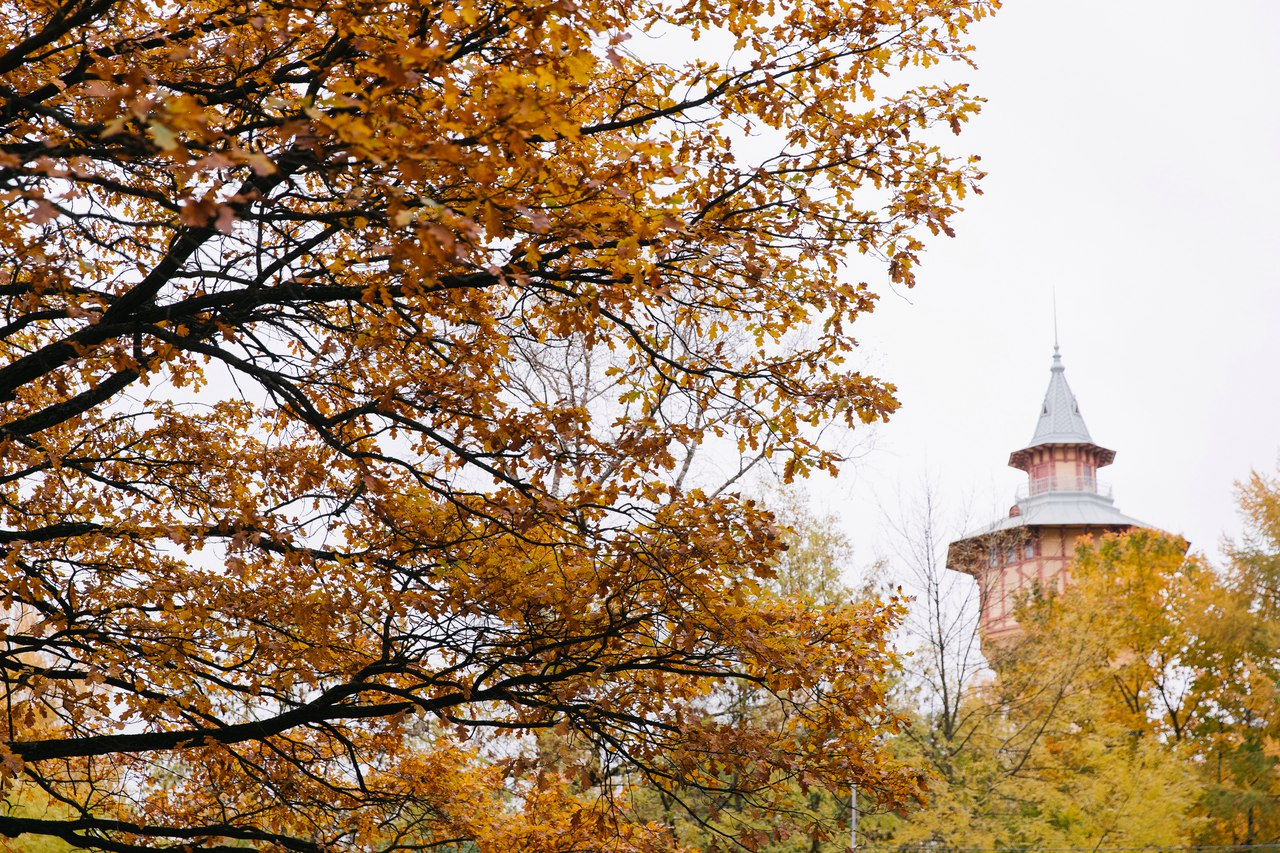
\includegraphics [scale=0.27] {my_folder/images//spbpu_hydrotower}
	\caption{Вид на гидробашню СПбПУ \cite{spbpu-gallery}} 
	\label{fig:spbpu_hydrotower}  
\end{figure}
%
%
%\begin{table} [htbp]% Пример оформления таблицы
%	\centering\small
%	\caption{Представление данных для сквозного примера по ВКР \cite{Peskov2004}}%
%	\label{tab:ToyCompare}		
%		\begin{tabular}{|l|l|l|l|l|l|}
%			\hline
%			$G$&$m_1$&$m_2$&$m_3$&$m_4$&$K$\\
%			\hline
%			$g_1$&0&1&1&0&1\\ \hline
%			$g_2$&1&2&0&1&1\\ \hline
%			$g_3$&0&1&0&1&1\\ \hline
%			$g_4$&1&2&1&0&2\\ \hline
%			$g_5$&1&1&0&1&2\\ \hline
%			$g_6$&1&1&1&2&2\\ \hline		
%		\end{tabular}	
%	\normalsize% возвращаем шрифт к нормальному
%\end{table}


% \firef{} от figure reference
% \taref{} от table reference
% \eqref{} от equation reference

На \firef{fig:spbpu_hydrotower} изображена гидробашня СПбПУ, а в \taref{tab:ToyCompare} приведены данные, на примере которых коротко и наглядно будет изложена суть ВКР.


\section{Название параграфа} \label{ch1:sec2} 



Формулы могут быть размещены в несколько строк. Чтобы выставить номер формулы напротив средней строки, используйте окружение \verb|multlined| из пакета \verb|mathtools| следующим образом \cite{Ganter1999}:
%
\begin{equation} 
\label{eq:fConcept-order-ch1}
\begin{multlined}
(A_1,B_1)\leq (A_2,B_2)\; \Leftrightarrow \\  \Leftrightarrow\; A_1\subseteq A_2\; \Leftrightarrow \\ \Leftrightarrow\; B_2\subseteq B_1. 
\end{multlined}
\end{equation}


Используя команду \verb|\labelcref| из пакета \verb|cleveref|, допустимо следующим образом оформлять ссылку на несколько формул:
(\labelcref{eq:Pi-ch1,eq:fConcept-order-ch1}).
%
%
На \firef{fig:spbpu_whitehall-three-photos} приведены три картинки под~общим номером и~названием, но с раздельной нумерацией подрисунков посредством пакета \verb|subcaption|.
%
\begin{figure}[!htbp]
	\adjustbox{minipage=1.3em,valign=t}{\subcaption{}\label{fig:spbpu_whitehall-a}}%
	\begin{subfigure}[t]{\dimexpr.3\linewidth-1.3em\relax}
		\centering
		
\includegraphics[width=.95\linewidth,valign=t]{my_folder/images//spbpu_whitehall}
	\end{subfigure}
	\hfill %выровнять
	\adjustbox{minipage=1.3em,valign=t}{\subcaption{}\label{fig:spbpu_whitehall-b}}%
	\begin{subfigure}[t]{\dimexpr.3\linewidth-1.3em\relax}
		\centering
		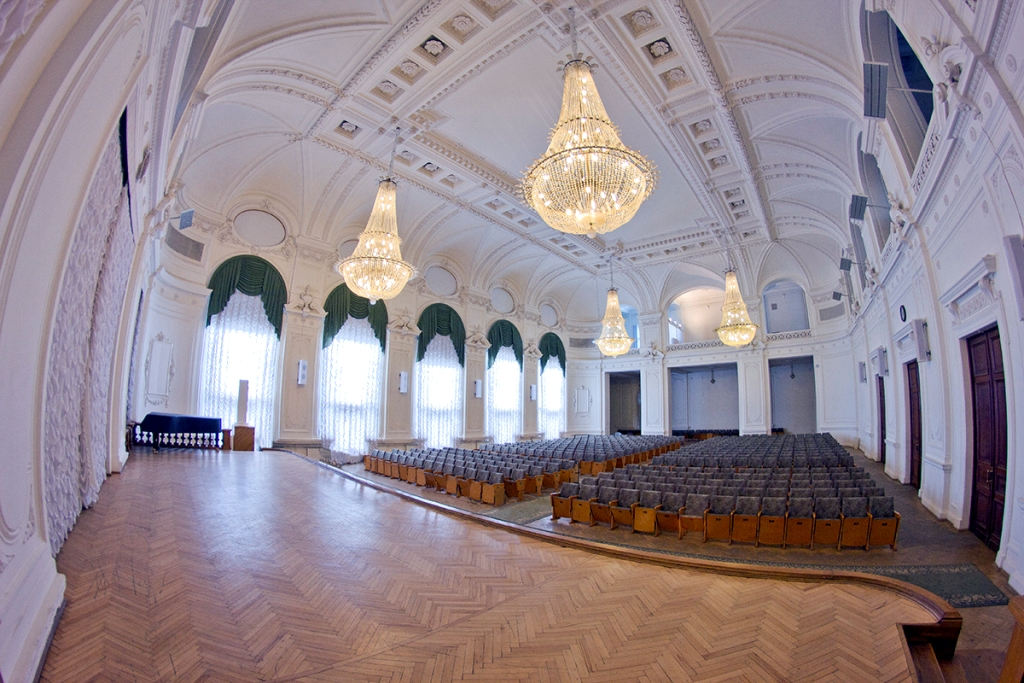
\includegraphics[width=.95\linewidth,valign=t]{my_folder/images//spbpu_whitehall_ligh}
	\end{subfigure}
	\hfill %выровнять
		\adjustbox{minipage=1.3em,valign=t}{\subcaption{}\label{fig:spbpu_whitehall-c}}%
	\begin{subfigure}[t]{\dimexpr.3\linewidth-1.3em\relax}
		\centering
		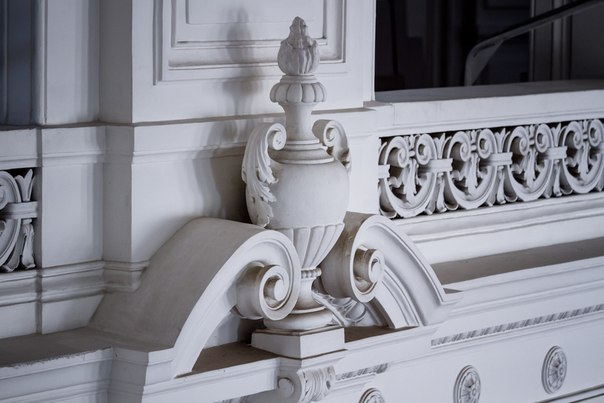
\includegraphics[width=.95\linewidth,valign=t]{my_folder/images//spbpu_whitehall_sculpture}
	\end{subfigure}%
\captionsetup{justification=centering} %центрировать
	\caption{Фотографии Белого зала СПбПУ \cite{spbpu-gallery}, в том числе: {\itshape a} --- со стороны зрителей; {\itshape b} --- со стороны сцены; {\itshape c} --- барельеф}\label{fig:spbpu_whitehall-three-photos}  
\end{figure}

Далее можно ссылаться на три отдельных рисунка: \firef{fig:spbpu_whitehall-a}, \firef{fig:spbpu_whitehall-b} и \firef{fig:spbpu_whitehall-c}. % пример подключения 3х иллюстрации в одном рисунке

Пример ссылок \cite{Article,Book,Booklet,Conference,Inbook,Incollection,Manual,Mastersthesis,Misc,Phdthesis,Proceedings,Techreport,Unpublished,badiou:briefings}, а также ссылок с указанием страниц, на котором отображены номера страниц  \cite[с.~96]{Naidenova2017} или в виде мультицитаты на несколько источников \cites[с.~96]{Naidenova2017}[с.~46]{Ganter1999}. Часть библиографических записей носит иллюстративный характер и не имеет отношения к реальной литературе. 



%\FloatBarrier % заставить рисунки и другие подвижные (float) элементы остановиться

\section{Выводы} \label{ch1:conclusion}

Текст выводов по главе \thechapter.

Кроме названия параграфа <<выводы>> можно использовать (единообразно по всем главам) следующие подходы к именованию последних разделов с результатами по главам:
\begin{itemize}
	\item <<выводы по главе N>>, где N --- номер соответствующей главы;
	\item <<резюме>>;
	\item <<резюме по главе N>>, где N --- номер соответствующей главы.
\end{itemize}

Параграф с изложением выводов по главе \textit{является обязательным}.

%% Вспомогательные команды - Additional commands
%
%\newpage % принудительное начало с новой страницы, использовать только в конце раздела
%\clearpage % осуществляется пакетом <<placeins>> в пределах секций
%\newpage\leavevmode\thispagestyle{empty}\newpage % 100 % начало новой страницы